\section{Introduzione}
In questa relazione si andrà ad esporre il procedimento per il dimensionamento di un muro a mensola, costruito in calcestruzzo armato.\\
Le opere di sostegno hanno la funzione di garantire una condizione di stabilità a volumi di terreno, nei casi in cui tale equilibrio non ci sarebbe. Una delle tipologie di opere di sostegno più utilizzate sono i muri, ovvero strutture con la funzione di contrastare le spinte (orizzontali o inclinate) trasmesse dal terreno, generalmente mediante il peso proprio del corpo.\\
Esistono diverse tipologie di muri, la cui scelta avverrà secondo diversi criteri tecnici, economici e funzionali, e sono: 
\begin{itemize}
    \item a gabbioni;
    \item a gravità;
    \item a mensola;
    \item a catasta;
    \item a contrafforti.
\end{itemize}
Il muro a mensola, rispetto quello a gravità, è molto più economico, poiché richiede l'utilizzo di meno cemento armato per la costruzione. Infatti, l'azione resistiva della struttura alle spinte esterne è prevalentemente dovuta al peso proprio del terreno.\\
L'utilizzo del cemento armato per la costruzione del muro a mensola permette alla struttura di resistere, entro certi limiti, sia alla forza compressiva (grazie alla resistenza del cemento) e sia alla forza di trazione (dovuta all'armatura in acciaio).\\
Le verifiche del muro sono state svolte mediante i criteri degli Stati Limite Ultimi (SLU) relativi alla geotecnica del suolo (GEO) ed alla struttura (STR), secondo le Norme Tecniche per le Costruzioni (NTC-2018).\\
\begin{figure}[H]
    \centering
    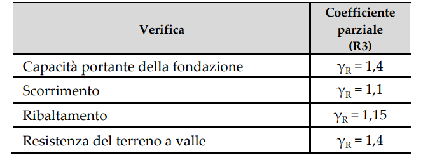
\includegraphics[width=0.6\textwidth]{immagini/coeff_parziali.png} \hfill
    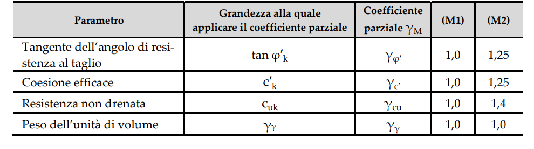
\includegraphics[width=0.6\textwidth]{immagini/parametri_geotecnici.png} \hfill
    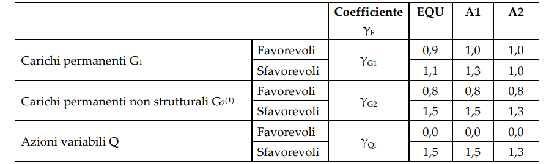
\includegraphics[width=0.6\textwidth]{immagini/verifiche_slu.png} \hfill
        \caption{Coefficienti per l'applicazione delle NTC-2018.}
    \label{figure:coeff_NTC2018}
\end{figure}
In particolare, le verifiche svolte riguardano il ribaltamento, lo scorrimento, il collasso della fondazione, la stabilità globale e la resistenza strutturale complessiva.\\
Il muro di cui è prevista la costruzione, presenta alcune specifiche di progetto, indicate nella seguente tabella.
\begin{table}[H] \centering
    \caption{Valori di progetto dell'opera.}
\begin{tabular}{ccc}
    \toprule
Altezza muro & H & 3 m \\
Resist. cilindrica caratteristica (cls) & $f_{ck}$ &  30 \unit{N/mm^2} \\
Peso specifico terreno & $\gamma_D$ &  18600 \unit{N/m^3} \\
Distanza lembo super. fondazione-piano campagna & $D_p$ & 0.4 \unit{m}  \\
Lunghezza muro & L & 10 \unit{m}  \\
Peso specifico cls & $\gamma_{CLS}$ & 25000 \unit{N/m^3}  \\
Angolo di resistenza al taglio del terreno & $\phi$ & 30°  \\
Carico distribuito sul terreno & q & 6000 \unit{N/m^2}  \\
    \bottomrule
\label{table:specifiche}
\end{tabular}

\end{table}
